Clase: 01/09/2022

\begin{nota}
    \begin{enumerate}
    \item Intuitivamente, el índice de una curva cerrada $\gamma$ es el número de veces que la curva gira con respecto a un punto.
    \item Sea $\gamma(t)=e^{it},0\leq t\leq 2\pi\implies \int_\gamma \frac{dz}{z}=2\pi i$
    $$\implies 1=\frac{1}{2\pi i}\int_\gamma \frac{dz}{z}.$$ Sea $\gamma(t)=e^{it},0\leq t\leq 2n\pi \implies \int_\gamma \frac{dz}{z}=2n\pi i$
    $$n=\frac{1}{2\pi i}\int_\gamma \frac{dz}{z}$$
    \item Sea $\tilde{\gamma}$ una curva cerrada que puede deformarse en $\gamma$ sin pasar por 0. 
    $$\int_{\tilde{\gamma}}\frac{dz}{z}=\int_\gamma \frac{dz}{z}$$
    $$\implies n=\frac{1}{2\pi i}\int_{\tilde{\gamma}}\frac{dz}{z}$$
\end{enumerate}
     
\end{nota}

\begin{definicion}
    Sea $\gamma$ una curva cerrada en $\mathbb{C}$ y sea $z_0\in \mathbb{C}\ni z_0\not\in \gamma$. El índice de $\gamma$ con respecto a $z_0$ es: 
    $$I(\gamma;z_0)=\frac{1}{2\pi i}\int_\gamma \frac{dz}{z-z_0}$$
\end{definicion}

\begin{teorema}
    Sea $\gamma:[a,b]\to\mathbb{C}$ una curva suave y cerrada, y sea $z_0\not\in\gamma$. Entonces, 
    $$I(\gamma;z_0)\in\mathbb{Z}$$
    \begin{proof}
        Sea $g(t):=\int_a^t\frac{\gamma'(s)}{\gamma(s)-z_0}ds\implies g'(t)=\frac{\gamma'(t)}{\gamma(t)-z_0}$. Nótese que: 
        \begin{align*}
            \frac{d}{dt}e^{-g(t)}\left[\gamma(t)-z_0\right] &=-e^{-g(t)}\cdot g'(t)\left[
                \gamma(t)-z_0\right] +e^{-g(t)}\cdot \gamma'(t)\\
                &= e^{-g(t)}\left[\gamma'(t)-g'(t)[\gamma(t)-z_0]\right]\\
                &= 0
        \end{align*}
        $\implies e^{-g(t)}[\gamma(t)-z_0]$ es constante sobre $[a,b]$. $\implies$ El valor de esta función es $e^{-g(a)}[\gamma(a)-z_0]\implies e^{-g(a)}[\gamma(a)-z_0]=e^{-g(b)}[\gamma(b)-z_0]\implies e^{-g(a)}=e^{-g(b)}$. Como $g(a)=0\implies e^{-g(b)}=1$. $\implies \pm g(b)$ debe ser un múltiplo entero de $2\pi i\implies g(b)=\int_a^b\frac{\gamma'(s)}{\gamma(s)-z_0}ds=\int\frac{dz}{z-z_0}=2n\pi i,n\in\mathbb{Z}$. Por lo tanto, 
        $$n=\frac{1}{2\pi i}\int_\gamma \frac{dz}{z-z_0}\in \mathbb{Z}$$
    \end{proof}
\end{teorema}

\begin{teorema}[Fórmula integral de Cauchy]
    Sea $f(z)$ una función analítica sobre y en el interior de una curva cerrada, suave y simple $\gamma$, que está sobre una región $R\subseteq \mathbb{C}$. Entonces, 
    $$f(a)=\frac{1}{2\pi i}\int_\gamma\frac{f(z)}{z-a}dz$$
    \begin{cajita}
        $$\iff \int_\gamma \frac{f(z)}{z-a}dz = f(a)2\pi i$$
    \end{cajita}
\end{teorema}

\begin{ejemplo}
    Calcule $\int_\gamma \frac{e^{z^2}}{z-2}dz$, donde $\gamma$ es: 
    \begin{figure}[H]
        \centering
        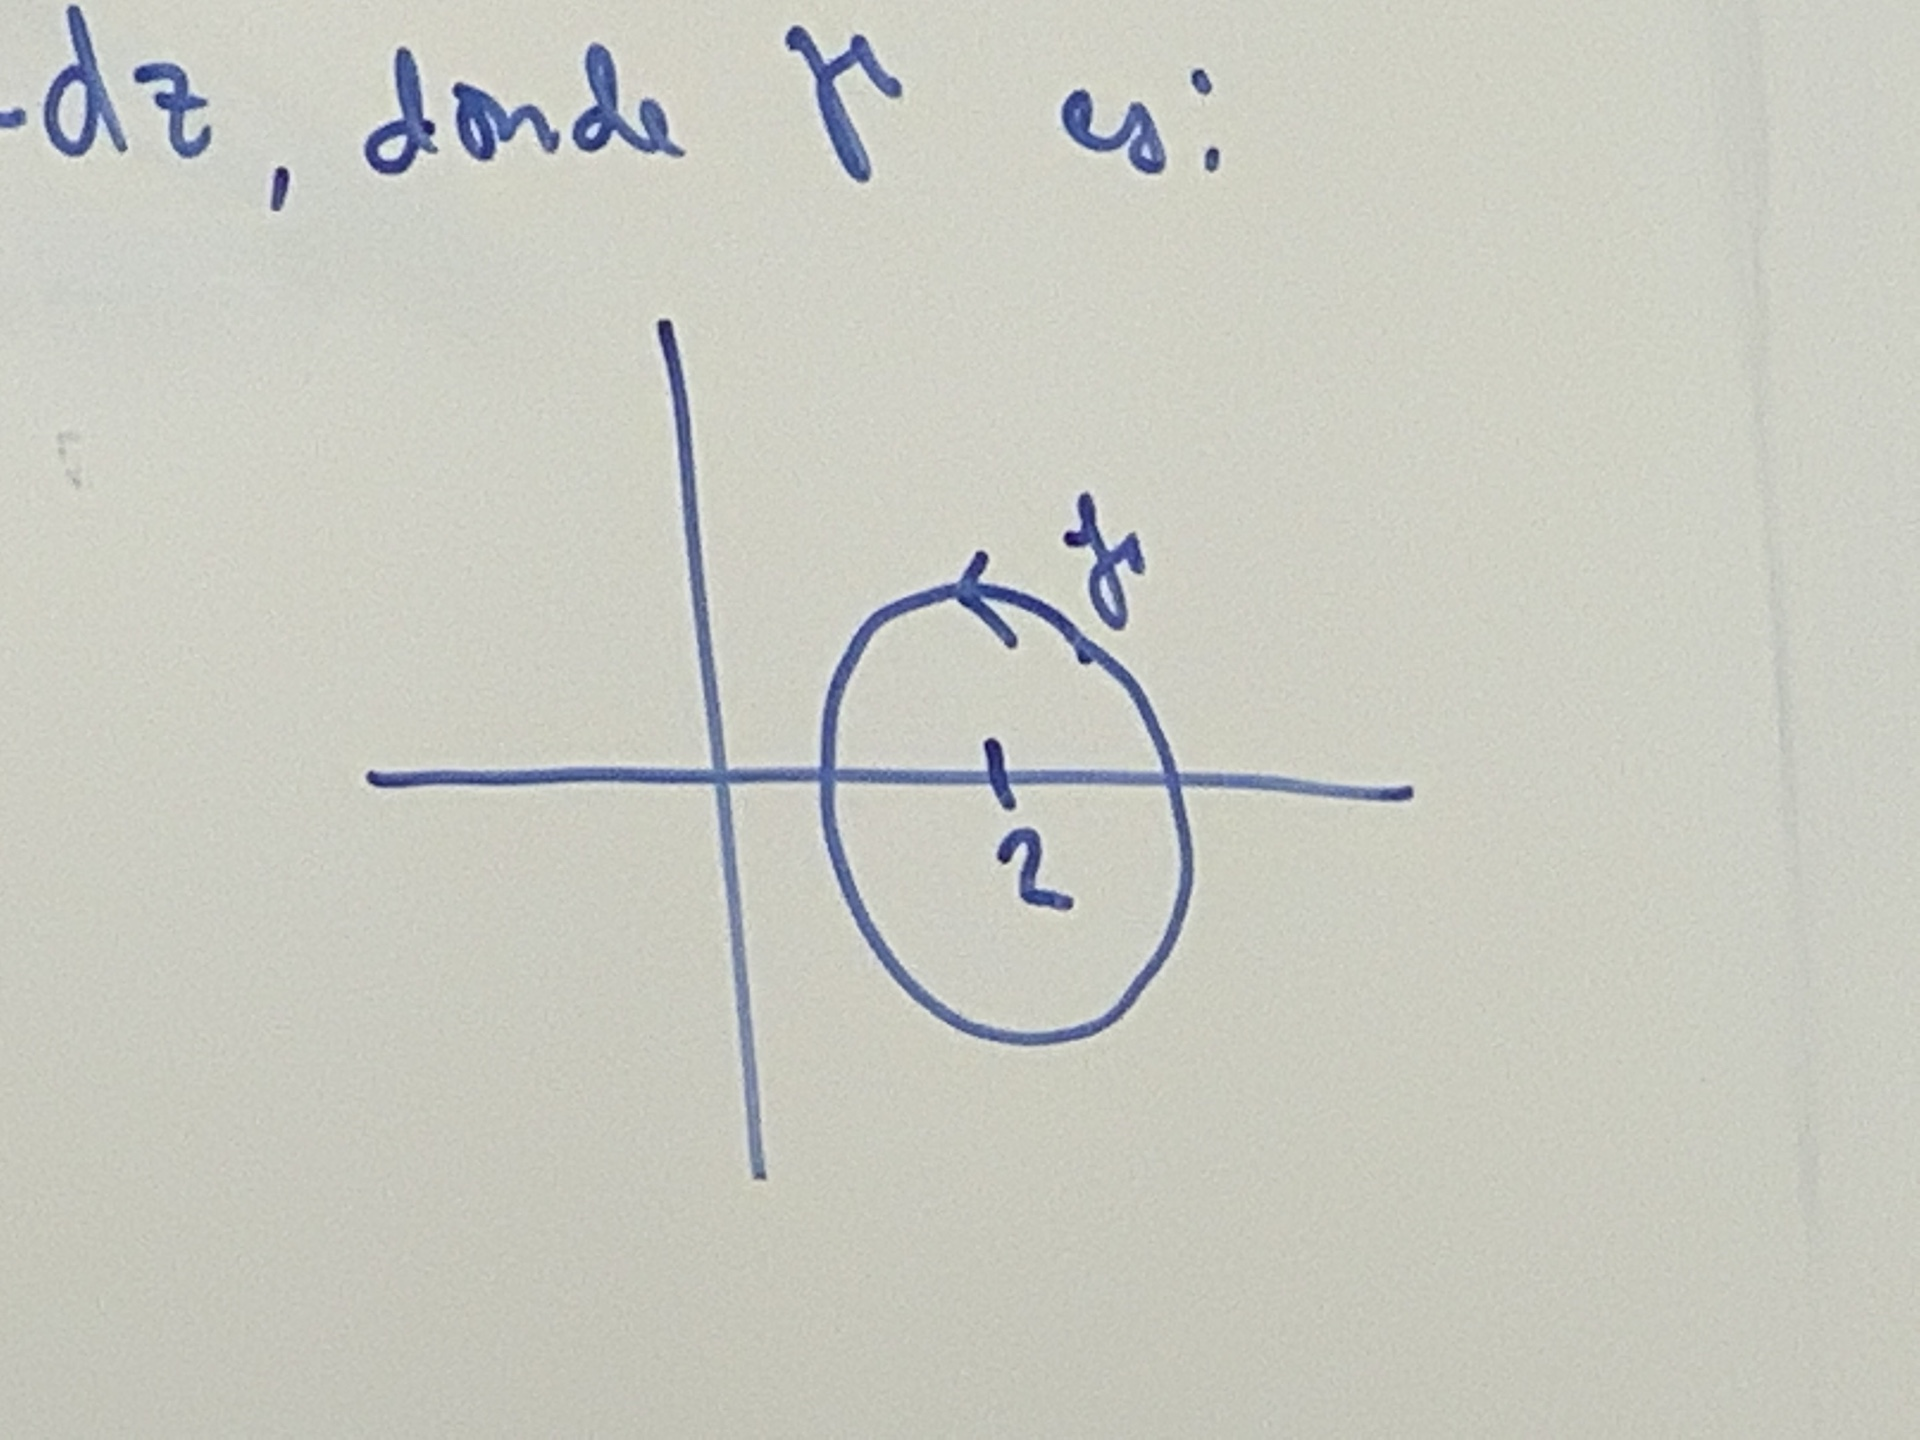
\includegraphics[scale=0.1]{imagenes/13.1.jpeg}
    \end{figure}
    $\implies \int_\gamma \frac{e^{z^2}}{z-2}dz =2\pi i[e^{(2)^2}]=2e^4\pi i$
    \begin{cajita}
        \begin{ejemplo}
            Calcule $\int_\gamma\frac{e^{z^2}}{z-2}dz$
            \begin{figure}[H]
                \centering
                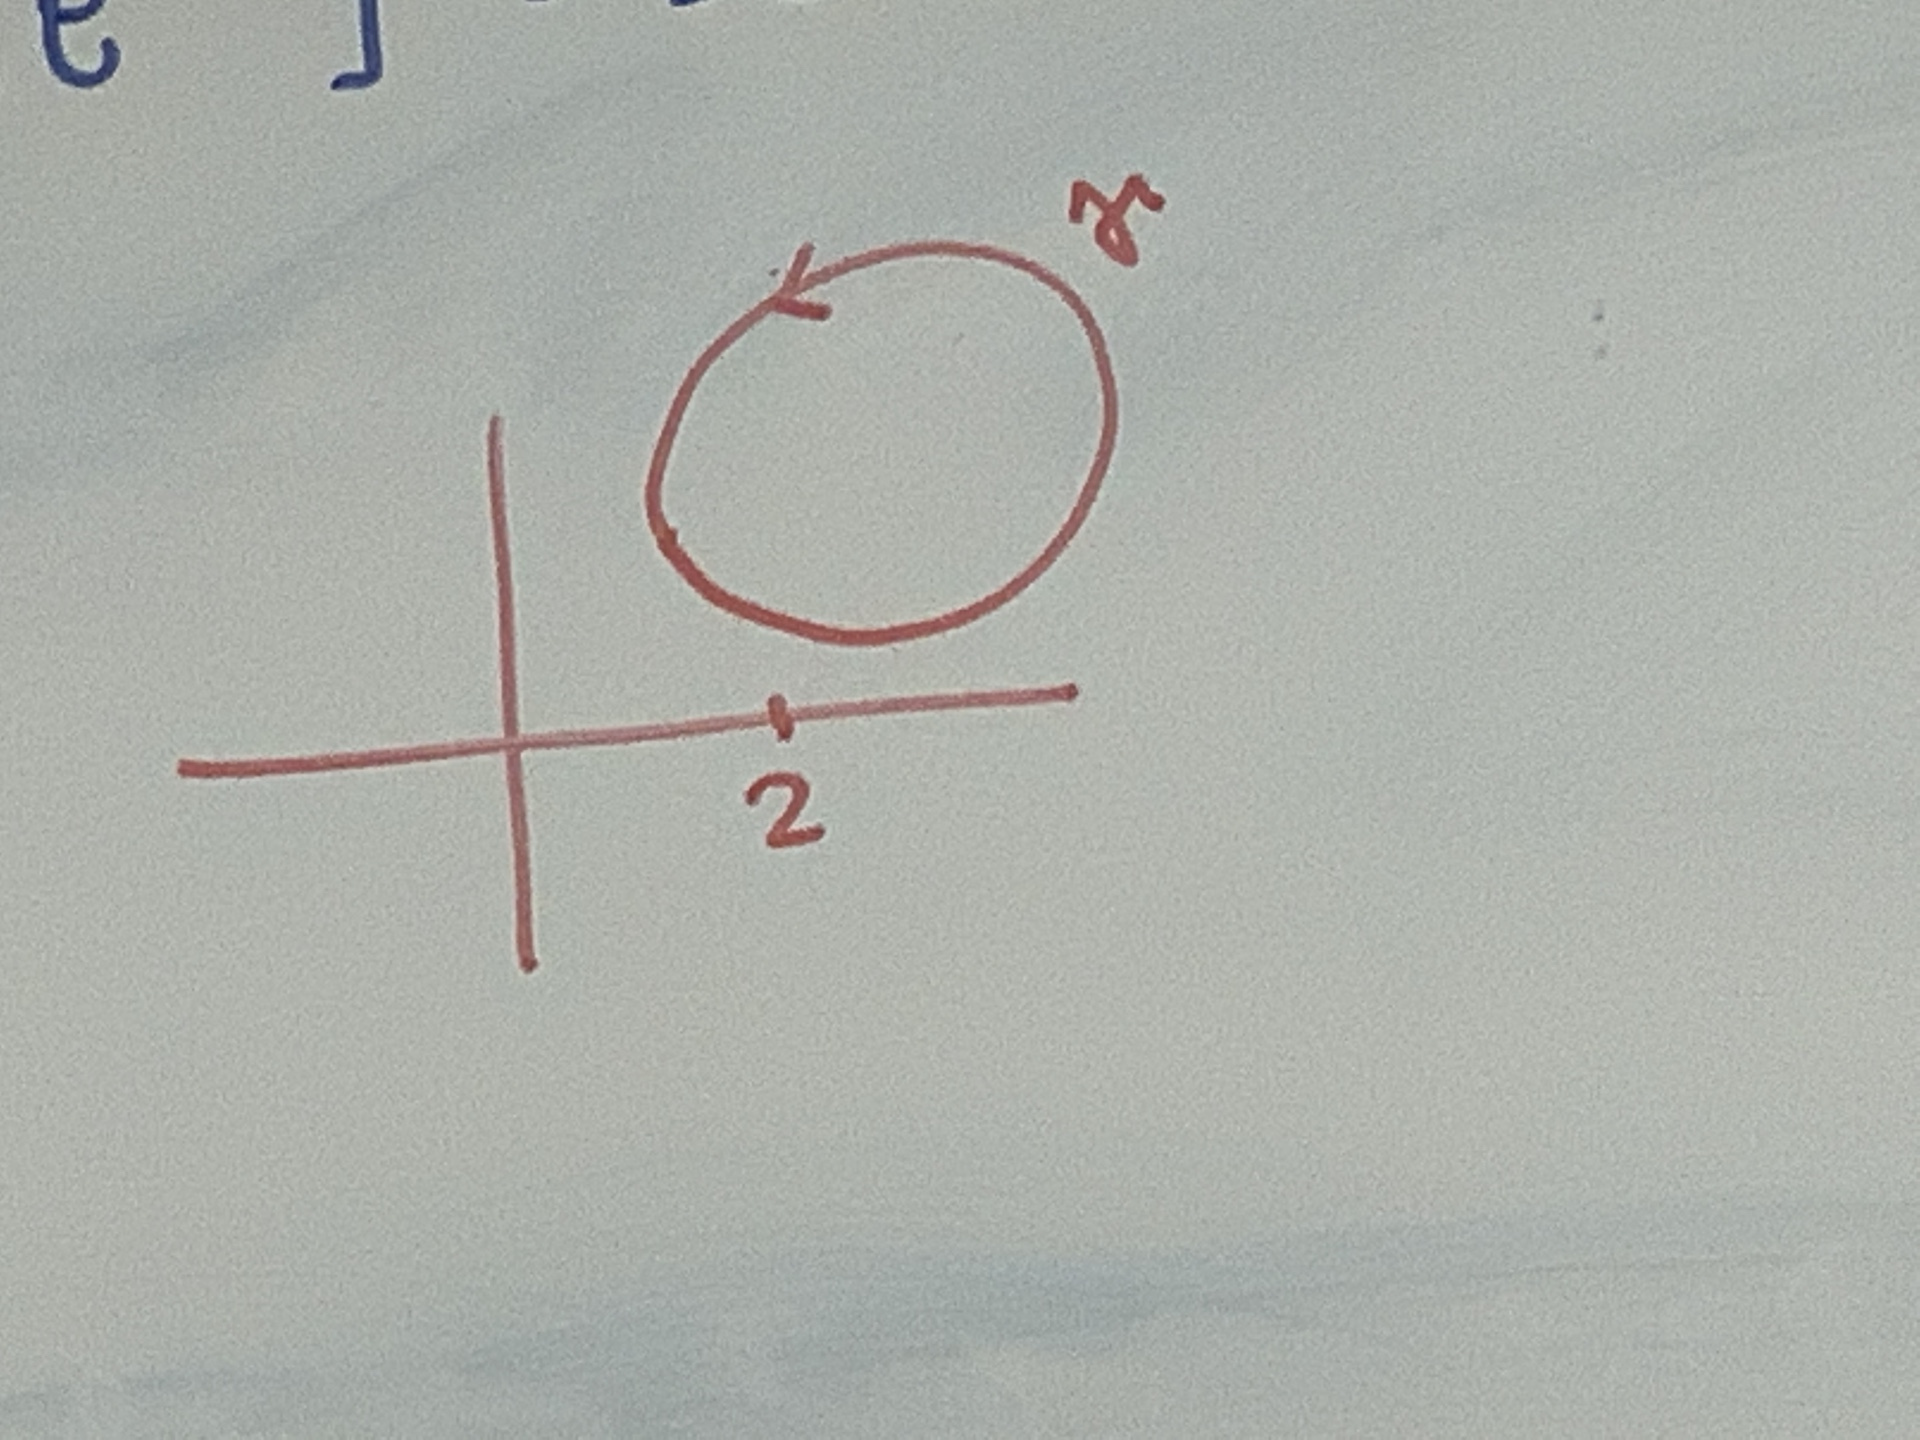
\includegraphics[scale=0.1]{imagenes/13.2.jpeg}
            \end{figure}
        \end{ejemplo}
    \end{cajita}
\end{ejemplo}

\begin{dem}
    Calculemos $\int_\gamma \frac{f(z)}{z-a}dz$. Sea $\gamma$ homotópica a $\tilde{\gamma}(z)=a+\varepsilon e^{it},0\leq t\leq 2\pi \implies \int_\gamma \frac{f(z)}{z-a}dz=\int_0^{2\pi}\frac{f(a+\varepsilon e^{it})}{a+\varepsilon e^{it}-a}\cdot\varepsilon ie^{it}dt=i\int_0^{2\pi}f(a+\varepsilon e^{it})dt$. Si $\varepsilon\to 0 i\ni \int_0^{2\pi}f(a)dt = 2\pi i f(a)$
\end{dem}

\begin{teorema}[Fórmula integral de Cauchy - Versión 2]
    Sea $F$ analítica sobre una región $R\subseteq \mathbb{C}$. Sea $\gamma$ una curva cerrada y suave en $R$ que es homotópica a un punto, y sea $z_0\in R, z_0\not\in \gamma$. Entonces, 
    $$f(z_0)\cdot I(\gamma;z_0)=\frac{1}{2\pi i}\int_\gamma \frac{f(z)}{z-z_0}dz$$ 
\end{teorema}

